% Fichier généré automatiquement par le notebook le 24/10/2026 15:19
\newcommand{\NbRep}{%
10%
}

\newcommand{\TabAcc}{%
\begin{table}[H]
\centering
\caption{Précision sur le test en \% (moyenne $\pm$ écart-type sur $R = 10$ répétitions). Meilleure moyenne en gras.}
\label{tab:acc}
\begin{tabular}{@{}lcccc@{}}
\toprule
Jeu de données & Toutes & Filtre & AG & BPSO \\
\midrule
Breast Cancer & $\mathbf{96{,}3 \pm 1{,}4}$ & $96{,}0 \pm 1{,}6$ & $96{,}0 \pm 1{,}8$ & $96{,}0 \pm 1{,}3$ \\
Sonar & $80{,}0 \pm 4{,}6$ & $77{,}6 \pm 5{,}4$ & $\mathbf{81{,}3 \pm 6{,}4}$ & $79{,}4 \pm 5{,}3$ \\
Ionosphere & $83{,}3 \pm 2{,}1$ & $86{,}8 \pm 5{,}0$ & $\mathbf{88{,}0 \pm 3{,}6}$ & $87{,}0 \pm 2{,}6$ \\
\bottomrule
\end{tabular}
\end{table}%
}

\newcommand{\TabNvar}{%
\begin{table}[H]
\centering
\caption{Nombre de variables sélectionnées $|S|$ (moyenne $\pm$ écart-type). Plus petite moyenne en gras (hors Toutes).}
\label{tab:nvar}
\begin{tabular}{@{}lcccc@{}}
\toprule
Jeu de données & Toutes & Filtre & AG & BPSO \\
\midrule
Breast Cancer & $30$ & $22{,}0 \pm 0{,}0$ & $\mathbf{13{,}3 \pm 3{,}2}$ & $14{,}3 \pm 1{,}9$ \\
Sonar & $60$ & $29{,}4 \pm 11{,}0$ & $\mathbf{25{,}9 \pm 3{,}8}$ & $28{,}5 \pm 4{,}0$ \\
Ionosphere & $34$ & $\mathbf{6{,}8 \pm 6{,}8}$ & $7{,}8 \pm 1{,}2$ & $9{,}5 \pm 2{,}1$ \\
\bottomrule
\end{tabular}
\end{table}%
}

\newcommand{\TabTemps}{%
\begin{table}[H]
\centering
\caption{Temps moyen de sélection par exécution (secondes) et rapport au temps du filtre.}
\label{tab:temps}
\begin{tabular}{@{}lccccc@{}}
\toprule
Jeu de données & Filtre & AG & BPSO & AG / Filtre & BPSO / Filtre \\
\midrule
Breast Cancer & $0{,}18$ & $10{,}33$ & $13{,}98$ & $\times 57$ & $\times 78$ \\
Sonar & $0{,}16$ & $7{,}09$ & $9{,}18$ & $\times 44$ & $\times 58$ \\
Ionosphere & $0{,}17$ & $9{,}66$ & $12{,}29$ & $\times 56$ & $\times 72$ \\
\bottomrule
\end{tabular}
\end{table}%
}

\newcommand{\TabWilcoxon}{%
\begin{table}[H]
\centering
\caption{Test de Wilcoxon apparié, bilatéral (valeurs $p$ ; en gras si $p < 0{,}05$).}
\label{tab:wilcoxon}
\small
\begin{tabular}{@{}lcccccc@{}}
\toprule
 & \multicolumn{2}{c}{AG vs BPSO} & AG vs Filtre & BPSO vs Filtre & AG vs Toutes & BPSO vs Toutes \\
\cmidrule(lr){2-3}\cmidrule(lr){4-4}\cmidrule(lr){5-5}\cmidrule(lr){6-6}\cmidrule(lr){7-7}
Jeu de données & précision & $|S|$ & précision & précision & précision & précision \\
\midrule
Breast Cancer & $0{,}863$ & $0{,}467$ & $1{,}000$ & $1{,}000$ & $0{,}266$ & $0{,}477$ \\
Sonar & $0{,}416$ & $0{,}160$ & $0{,}258$ & $0{,}242$ & $0{,}523$ & $0{,}438$ \\
Ionosphere & $0{,}391$ & $\mathbf{0{,}008}$ & $0{,}586$ & $1{,}000$ & $\mathbf{0{,}004}$ & $\mathbf{0{,}004}$ \\
\bottomrule
\end{tabular}
\end{table}%
}

\newcommand{\FigConvergence}{%
\begin{figure}[H]
\centering
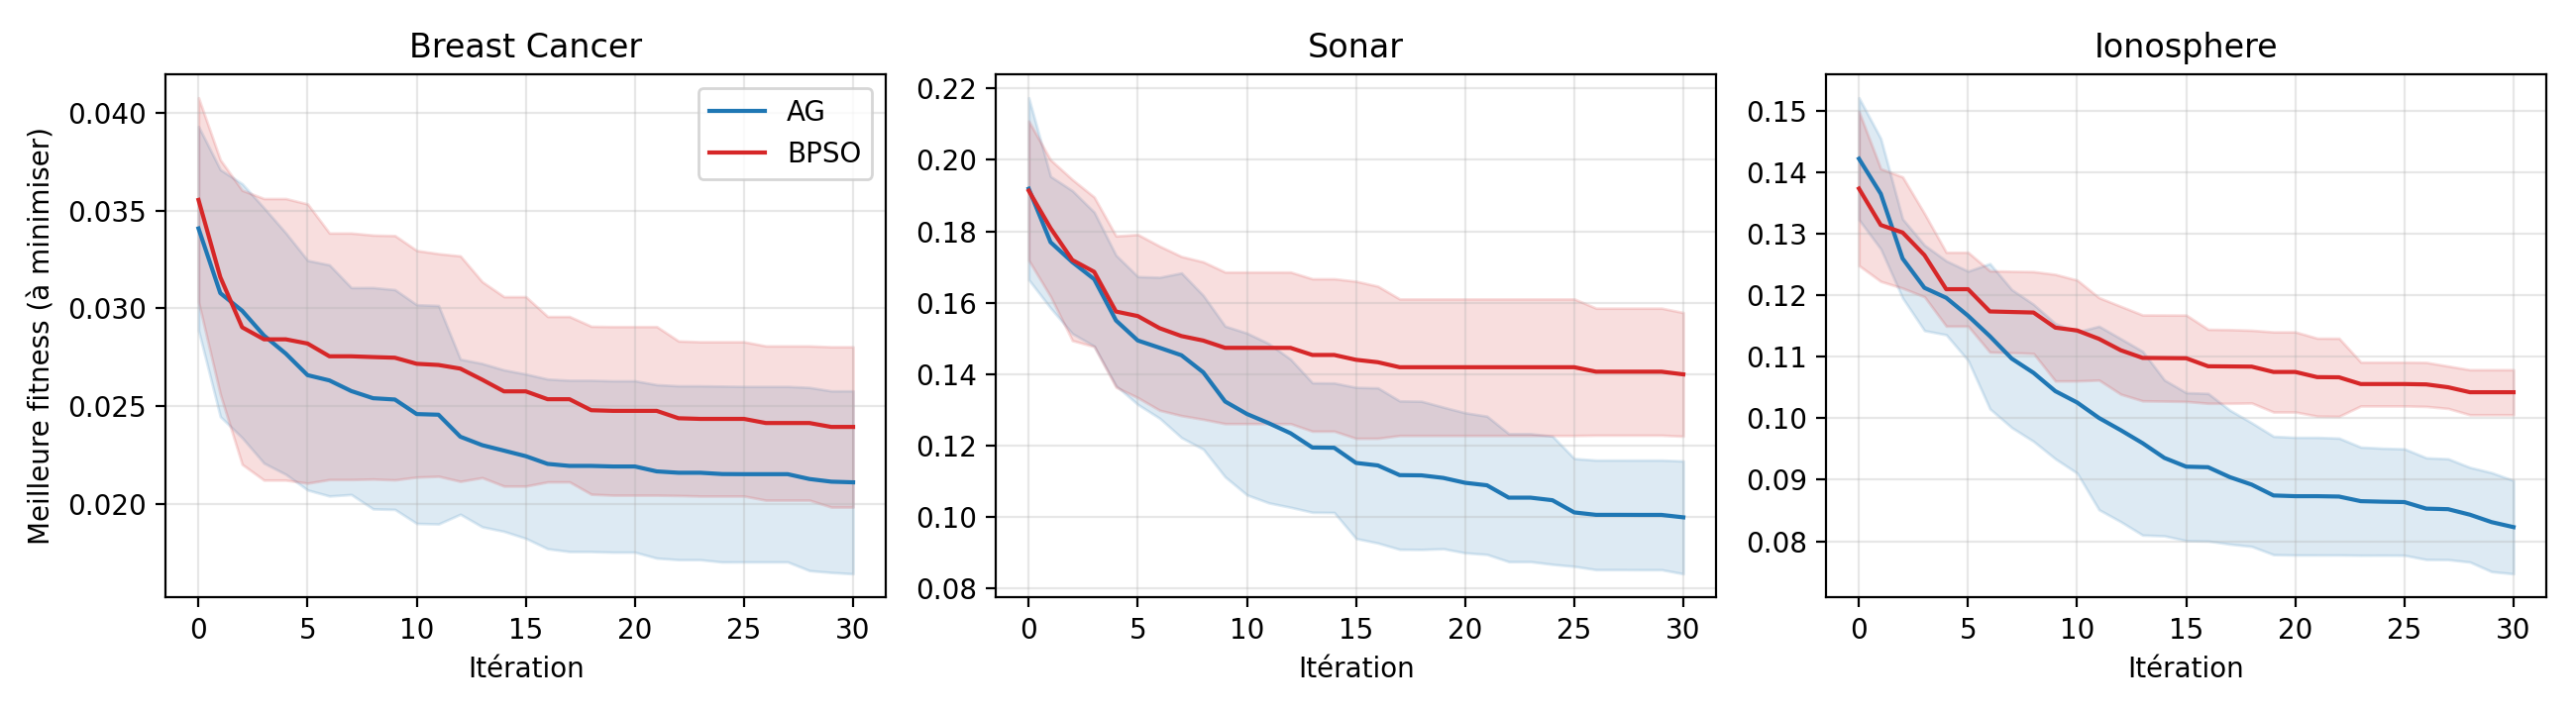
\includegraphics[width=\linewidth]{figures/convergence.png}
\caption{Convergence : meilleure fitness moyenne par itération ($\pm$ écart-type, 10 répétitions).}
\label{fig:convergence}
\end{figure}%
}

\newcommand{\FigBoxplot}{%
\begin{figure}[H]
\centering
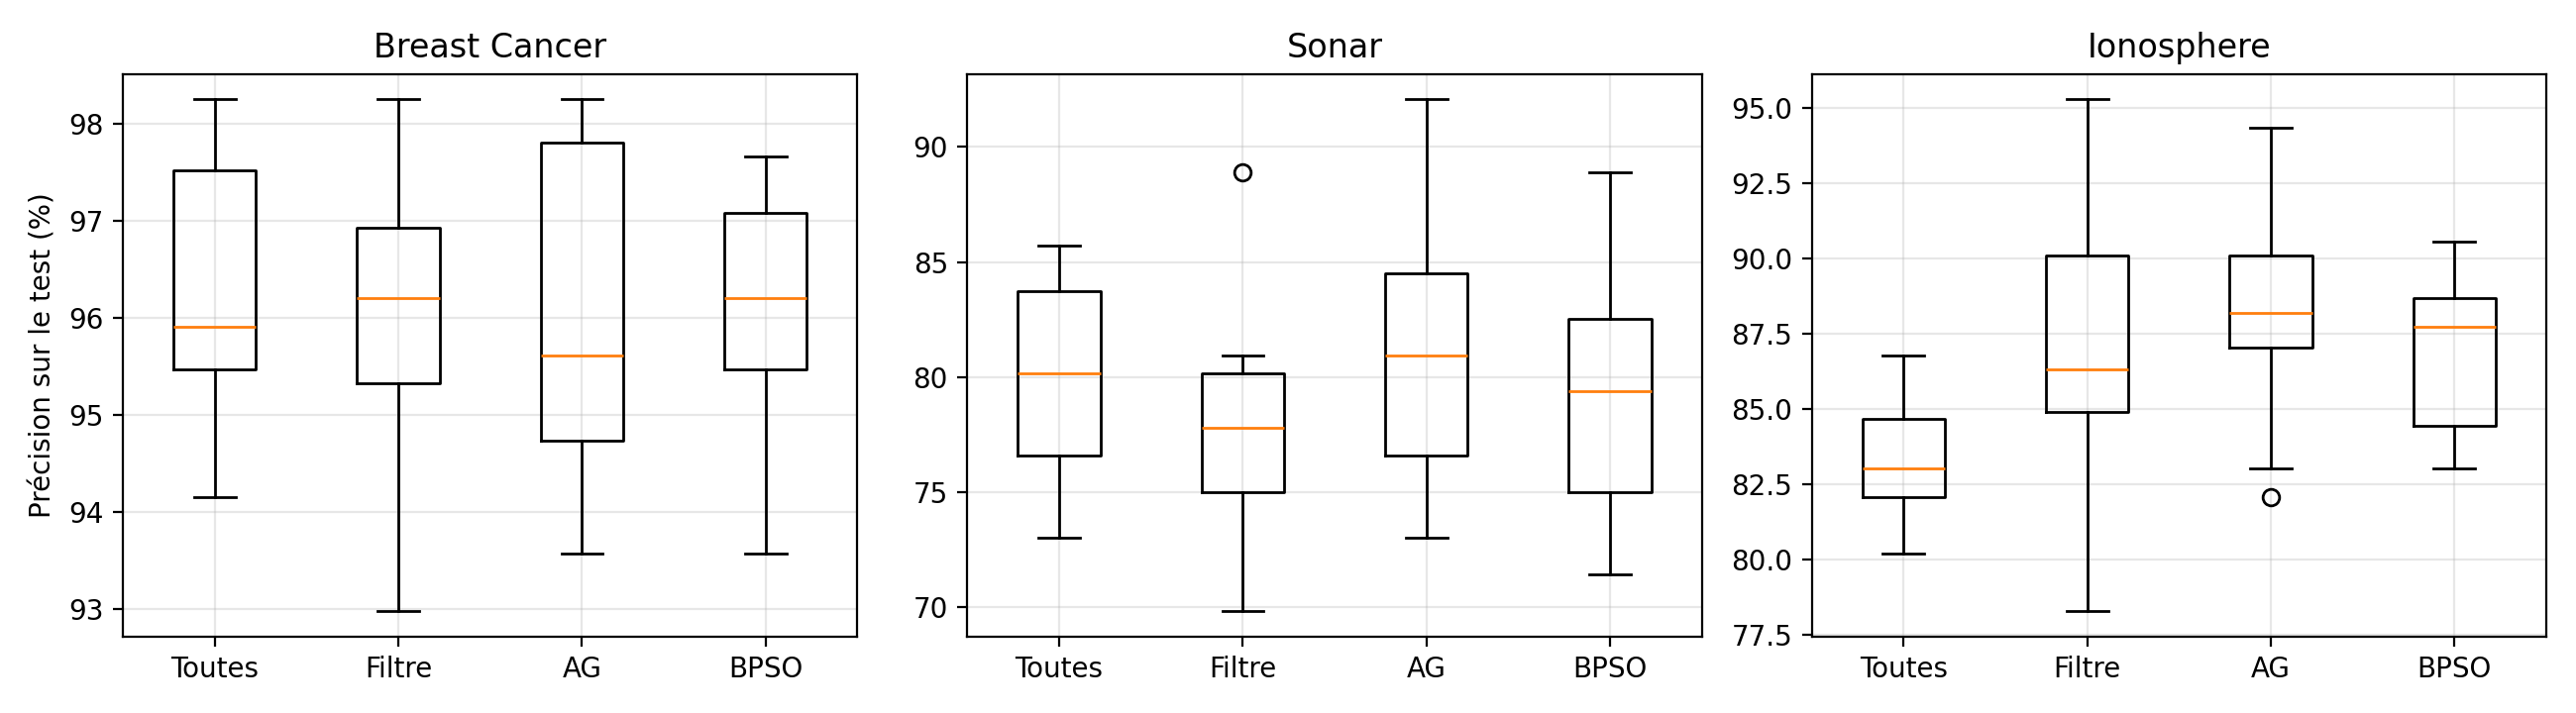
\includegraphics[width=\linewidth]{figures/boxplot_precision.png}
\caption{Distribution de la précision sur le test sur les 10 répétitions.}
\label{fig:boxplot}
\end{figure}%
}

\newcommand{\ResPrecision}{%
Sur Breast Cancer, la meilleure précision moyenne est obtenue par la référence Toutes (96{,}3~\%). Par rapport à l'utilisation de toutes les variables (96{,}3~\%), l'écart est de $-0{,}4$~point pour l'AG, $-0{,}3$~point pour le BPSO et $-0{,}4$~point pour le filtre.
Sur Sonar, la meilleure précision moyenne est obtenue par l'AG (81{,}3~\%). Par rapport à l'utilisation de toutes les variables (80{,}0~\%), l'écart est de $+1{,}3$~point pour l'AG, $-0{,}6$~point pour le BPSO et $-2{,}4$~points pour le filtre.
Sur Ionosphere, la meilleure précision moyenne est obtenue par l'AG (88{,}0~\%). Par rapport à l'utilisation de toutes les variables (83{,}3~\%), l'écart est de $+4{,}7$~points pour l'AG, $+3{,}7$~points pour le BPSO et $+3{,}5$~points pour le filtre.
Les écarts-types de la précision varient de 1{,}3 à 6{,}4~points selon la méthode et le jeu de données (tableau~\ref{tab:acc}, figure~\ref{fig:boxplot}).%
}

\newcommand{\ResVariables}{%
Sur Breast Cancer ($N = 30$), l'AG retient en moyenne 13{,}3 variables (44~\% de $N$), le BPSO 14{,}3 (48~\%) et le filtre 22{,}0 (73~\%).
Sur Sonar ($N = 60$), l'AG retient en moyenne 25{,}9 variables (43~\% de $N$), le BPSO 28{,}5 (48~\%) et le filtre 29{,}4 (49~\%).
Sur Ionosphere ($N = 34$), l'AG retient en moyenne 7{,}8 variables (23~\% de $N$), le BPSO 9{,}5 (28~\%) et le filtre 6{,}8 (20~\%).
L'écart-type moyen de $|S|$ entre répétitions est de 2{,}7 pour l'AG, 2{,}7 pour le BPSO et 5{,}9 pour le filtre (tableau~\ref{tab:nvar}).%
}

\newcommand{\ResTemps}{%
Le filtre sélectionne les variables en 0{,}16 à 0{,}18~s selon le jeu de données. La sélection par AG est 44 à 57 fois plus lente, et celle par BPSO 58 à 78 fois plus lente (tableau~\ref{tab:temps}).
À budget égal, le BPSO est plus lent que l'AG sur les trois jeux de données.
Le nombre d'évaluations étant identique, cet écart provient surtout du nombre de sous-ensembles distincts réellement évalués (la mémoïsation évite de réentraîner un masque déjà vu) et de la taille des sous-ensembles évalués.%
}

\newcommand{\ResSignif}{%
Sur Breast Cancer, la différence de précision entre AG et BPSO n'est pas significative ($p = 0{,}863$), et celle du nombre de variables n'est pas significative ($p = 0{,}467$). Par rapport au filtre, la différence de précision de l'AG n'est pas significative ($p = 1{,}000$) ; celle du BPSO n'est pas significative ($p = 1{,}000$).
Sur Sonar, la différence de précision entre AG et BPSO n'est pas significative ($p = 0{,}416$), et celle du nombre de variables n'est pas significative ($p = 0{,}160$). Par rapport au filtre, la différence de précision de l'AG n'est pas significative ($p = 0{,}258$) ; celle du BPSO n'est pas significative ($p = 0{,}242$).
Sur Ionosphere, la différence de précision entre AG et BPSO n'est pas significative ($p = 0{,}391$), et celle du nombre de variables est significative ($p = 0{,}008$). Par rapport au filtre, la différence de précision de l'AG n'est pas significative ($p = 0{,}586$) ; celle du BPSO n'est pas significative ($p = 1{,}000$).
Avec $R = 10$ répétitions, la plus petite valeur $p$ atteignable par le test de Wilcoxon bilatéral exact est d'environ $0{,}002$ (tableau~\ref{tab:wilcoxon}).%
}

\newcommand{\ResConvergence}{%
Sur Breast Cancer, l'AG atteint la meilleure fitness moyenne finale (AG : 0{,}0211 ; BPSO : 0{,}0239). L'AG réalise 95~\% de son amélioration totale à l'itération 21, le BPSO à l'itération 22.
Sur Sonar, l'AG atteint la meilleure fitness moyenne finale (AG : 0{,}0999 ; BPSO : 0{,}1399). L'AG réalise 95~\% de son amélioration totale à l'itération 25, le BPSO à l'itération 17.
Sur Ionosphere, l'AG atteint la meilleure fitness moyenne finale (AG : 0{,}0823 ; BPSO : 0{,}1042). L'AG réalise 95~\% de son amélioration totale à l'itération 27, le BPSO à l'itération 23.
La courbe moyenne de l'AG décroît encore au cours des cinq dernières itérations sur Breast Cancer, Sonar et Ionosphere, ce qui suggère qu'un budget plus élevé pourrait encore l'améliorer.
La courbe moyenne du BPSO décroît encore au cours des cinq dernières itérations sur Breast Cancer, Sonar et Ionosphere, ce qui suggère qu'un budget plus élevé pourrait encore l'améliorer.
(Figure~\ref{fig:convergence}.)%
}

\newcommand{\DiscHypotheses}{%
\textbf{H1 est confirmée} sur les trois jeux de données. Critère : sur un jeu de données, H1 est vérifiée si la précision de l'AG et du BPSO n'est pas significativement inférieure à celle de la référence Toutes et si chacun retient au plus la moitié des variables (tableaux~\ref{tab:acc}, \ref{tab:nvar} et \ref{tab:wilcoxon}).

\textbf{H2 est confirmée}. L'écart de précision entre la meilleure métaheuristique et le filtre vaut $+0{,}1$~point sur Breast Cancer, $+3{,}7$~points sur Sonar, $+1{,}2$~point sur Ionosphere ; il est le plus grand sur Sonar, qui est bien le jeu de plus grande dimension ($N = 60$).

\textbf{H3 est confirmée}. Le plus petit rapport de temps observé entre une métaheuristique et le filtre est de 44 (tableau~\ref{tab:temps}) ; le seuil d'un ordre de grandeur correspond à un rapport de 10.

\textbf{H4 est confirmée au sens faible} : le BPSO n'est significativement moins précis que l'AG sur aucun jeu de données (sa précision moyenne est supérieure ou égale sur 1 des 3 jeux), mais aucune différence n'est significative.%
}

\newcommand{\DiscLitterature}{%
Babaoğlu et al.~\cite{babaoglu2010} et Rafdi et al.~\cite{rafdi2021} rapportent un avantage du BPSO sur l'AG, chacun sur un seul jeu de données. Nos résultats nuancent cette tendance : à budget égal et sur trois jeux de données, aucune différence de précision entre AG et BPSO n'est statistiquement significative. L'avantage rapporté dans ces études, obtenu sur un seul jeu de données, ne se généralise donc pas ici.%
}

\newcommand{\DiscEcart}{%
Sur l'ensemble des répétitions, pour l'AG, la précision estimée en validation croisée sur l'apprentissage dépasse la précision mesurée sur le test de 5{,}1~points en moyenne ; pour le BPSO, la précision estimée en validation croisée sur l'apprentissage dépasse la précision mesurée sur le test de 3{,}9~points en moyenne. Cet écart positif montre que la fitness optimisée est une estimation optimiste : à force d'évaluer des centaines de sous-ensembles sur les mêmes plis, la recherche finit par exploiter des particularités de l'ensemble d'apprentissage. C'est précisément pour mesurer ce phénomène que la précision est rapportée sur un ensemble de test jamais utilisé pendant la sélection \cite{ambroise2002,kohavi1997}.%
}

\newcommand{\ReponseQuestion}{%
Dans nos conditions expérimentales, l'AG n'améliore significativement la précision du filtre sur aucun jeu de données, alors que sa sélection est 44 à 57 fois plus lente : du point de vue de la précision, son coût de calcul n'est pas justifié.%
}

\newcommand{\ResumeChiffres}{%
Sur Sonar (60 variables), l'AG atteint 81{,}3~\% de précision avec 25{,}9 variables en moyenne, le BPSO 79{,}4~\% avec 28{,}5 variables et le filtre 77{,}6~\% avec 29{,}4 variables, contre 80{,}0~\% avec toutes les variables ; la sélection par AG est 44 fois plus lente que le filtre. Dans nos conditions expérimentales, l'AG n'améliore significativement la précision du filtre sur aucun jeu de données, alors que sa sélection est 44 à 57 fois plus lente : du point de vue de la précision, son coût de calcul n'est pas justifié.%
}

\newcommand{\AbstractNumbers}{%
On Sonar (60 features), the GA reaches 81.3\% accuracy with 25.9 features on average, BPSO 79.4\% with 28.5 features and the filter 77.6\% with 29.4 features, versus 80.0\% with all features; GA selection is 44 times slower than the filter. Under our experimental conditions, the GA does not significantly improve on the filter's accuracy on any dataset, while being 44 to 57 times slower: in terms of accuracy, its computational cost is not justified.%
}

\newcommand{\ConclusionChapitre}{%
Les résultats établissent les points suivants : H1 est confirmée, H2 est confirmée, H3 est confirmée et H4 est confirmée au sens faible. Dans nos conditions expérimentales, l'AG n'améliore significativement la précision du filtre sur aucun jeu de données, alors que sa sélection est 44 à 57 fois plus lente : du point de vue de la précision, son coût de calcul n'est pas justifié.%
}

\newcommand{\Environnement}{%
Les expériences ont été réalisées sous Python 3.13.16 avec NumPy 2.1.3 et scikit-learn 1.6.1 (Google Colab, processeur x86\_64, 2 cœurs). La durée totale des expériences est d'environ 11~min.%
}

